\section{Materiali e Strumentazione}
La tecnica sperimentale impiegata per analizzare l'effetto Compton prevede di far incidere un fascio di fotoni, emesso da una sorgente radioattiva, su un bersaglio che serve da scatteratore. I fotoni prodotti e i fotoni scatterati sono rilevati attraverso due scintillatori. Il primo funge da gate e conteggio, il secondo, posto a vari angoli rispetto ai fotoni incidenti serve da spettrometro.
\subsection{Sorgente}
I due fotoni sono prodotti attraverso il decadimento $\beta^+$ della sorgente radioattiva $\ch{^{22}Na}$\footnote{Tutti i dati sono presi da: \url{https://nds.iaea.org/relnsd/vcharthtml/VChartHTML.html}}. ($\mathrm{BR}=89.90\,\%$, $t_{1/2}=2.6\,\mathrm{yr}$). 
\begin{equation}
    \ch{^{22}Na}\,\to\,\ch{^{22}Ne^*}+e^++\nu_e
\end{equation}
 %IMMAGINE sodiodecay
\begin{figure}[htp!]
  \centering
  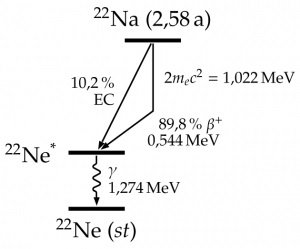
\includegraphics[scale=0.6]{Strumenti/sodiodecay.jpg} 
  \caption{Qui è possibile visualizzare in maniera schematica le due modalità di decadimento del $\ch{^{22}Na}$ e il diseccitamento elettromagnetico del $\ch{^{22}Ne^*}$}
\end{figure}
%va ridisegnato lo schema in quanto dal sito: https://nds.iaea.org/relnsd/vcharthtml/VChartHTML.html sono presenti dati leggermente diversi
La sorgente è sigillata all'interno di un involucro che induce tutti i positroni all'annichilazione con gli elettroni presenti nel materiale. La radiazione risultante è l'emissione di due $\gamma$ back to back con un'energia fissa di $511\,\unit{\kilo\electronvolt}$.
\begin{equation}
    e^++e^-\,\to\,2\gamma\,(511\,\unit{\kilo\electronvolt})
\end{equation}
La diseccitazione elettromagnetica del nucleo di $\ch{^{22}Ne^*}$ avviene in $t=3.6\,\unit{ps}$ con l'emissione di un $\gamma$ di energia $1274\,\unit{keV}$.
\begin{equation}
    \ch{^{22}Ne^*}\,\to\,\ch{^{22}Ne}+\gamma\,(1274\,\unit{keV})
\end{equation}
Oltre al decadimento $\beta^+$ è anche possibile la cattura elettronica con: $\mathrm{BR}=10.04\,\%$
\begin{equation}
    \ch{^{22}Na}+e^-\,\to\,\ch{^{22}Ne^*}+\nu_e
\end{equation}
L'attività della sorgente corrisponde a: $A=100,\unit{kBq}$.


Ricapitolando per ogni decadimento $\beta$ vengono emessi tre fotoni: i due provenienti dall'annichilazione di elettrone e positrone sono correlati in energie e direzione mentre il terzo è emesso in contemporanea ma in direzione casuale. L'emissione di due fotoni in direzione opposta alla stessa energia è una caratteristica fondamentale che rende possibile l'esecuzione della misura di coincidenza temporale tramite i due rivelatori: il rivelatore che svolge la funzione di spettrometro (indicato con A) e il secondo rilevatore (indicato con B) posizionato in direzione opposta allo scatteratore. 
\subsection{Rivelatori}
Il setup sperimentale è costituito da due scintillatori cilindrici inorganici. Il primo è uno scintillatore al cristallo di bromuro di cerio $\ch{CeBr_3}$ (usato come spettrometro e indicato con A), mentre il secondo è ai cristalli di ioduro di sodio $\ch{NaI}$ (usato come gate e indicato con B). Per quanto riguarda il secondo scintillatore è stato usato un drogante al tallio $\ch{Tl}$ il quale aggiunge livelli energetici ammessi all'interno della banda di energia proibita. Questi livelli in più hanno una doppia funzione: la prima è facilitare la ricombinazione elettrone-lacuna e la seconda è ridurre l'energia dell'emissione di luce rispetto a quella della bandgap. Entrambi gli scintillatori sono accoppiati a un fotomoltiplicatore.

Nella seguente tabella è possibile osservare le principali caratteristiche dei due scintillatori utilizzati:
\begin{table}[H]
    \centering
    \begin{tabular}{|c|c|c|c|c|c|}
    \hline
       Scintillatore  & $\rho$ $[\unit{g}/\unit{cm^3}]$ & $\lambda$ $[\unit{nm}]$ & $\tau$ $[\unit{ns}]$ & L.Y. $[\gamma/\unit{keV}]$ & $\Delta E/E$ $[\%]$ \\
    \hline
    \hline
    $\ch{CeBr_3}$ & $5.2$ & $380$ & $18$ & $45$ & $5$ \\
    \hline
    $\ch{NaI}:\ch{Tl}$ & $3.7$ & $415$ & $230$ & $38$ & $6$ \\
    \hline
    \end{tabular}
    \caption{Sono presentati i vari valori indicativi delle caratteristiche principali dei due scintillatori utilizati, senza errori corrispondenti.}
    \label{tab:scintillatori}
\end{table}

\subsection{Elettronica nucleare}\label{Elettronica nucleare}
Per riuscire a misurare e digitalizzare il segnale viene usata una catena elettronica divisa in diversi stadi. Lo schema dell'elettronica è presente nella figurag(\ref{fig:elettronica}). Quando la radiazione ionizzante interagisce con lo scintillatore, essa perde energia tramite processi come l'effetto fotoelettrico e l'effetto Compton. Gli elettroni generati da queste interazioni ionizzano il cristallo e, durante la ricombinazione con le lacune, vengono emessi numerosi fotoni, che ricadono generalmente nella banda del visibile. La quantità di fotoni emessi è proporzionale all'energia rilasciata dalla radiazione ionizzante. Una proprietà fondamentale dello scintillatore è il rendimento luminoso ($L_y$), espresso in termini di fotoni per $\unit{\kilo\electronvolt}$ ($\gamma/\unit{\kilo\electronvolt}$). 

Successivamente, i fotoni a bassa energia colpiscono il fotomoltiplicatore collegato al rivelatore. Questo processo estrae i primi elettroni dal fotocatodo, con una determinata efficienza quantica. Gli elettroni generati vengono quindi accelerati da un campo elettrico e colpiscono il primo elettrodo, chiamato dinodo, avviando una cascata di produzione di ulteriori elettroni. Infine, il segnale viene raccolto dall'anodo. Il segnale in uscita dipende dalla tensione di alimentazione del fototubo. 

Il segnale, trasportato attraverso cavi di tipo BNC, viene poi amplificato elettronicamente da uno stadio di preamplificazione in cui è importante fare attenzione al rapporto tra segnale e rumore. Il segnale amplificato viene trasferito in un amplificatore formatore necessario a dare la forma adatta per essere misurato massimizzando il rapporto segnale rumore. L'altezza dell'impulso viene misurata da un analizzatore multicanale (MCA). Questo dispositivo elettronico campiona il segnale al suo valore massimo e crea un istogramma, che mostra la distribuzione del numero di segnali campionati nei vari intervalli di ampiezza. Ogni canale dell'MCA corrisponde a un intervallo di tensione. Il campionamento del segnale avviene solo quando l'ampiezza del segnale in ingresso supera una soglia regolabile.

Per lo scopo di questo esperimento il rivelatore A è messo in coincidenza con il rivelatore B che funziona da Gate. Questo significa che quando dal software MAESTRO viene impostata la funzione di coincidenza gli unici segnali che vengono digitalizzati sono quelli in coincidenza con l'apertura del gate. Una descrizione più approfondita verrà fatta nella sezione dedicata alla calibrazione (\ref{Sez calibrazione}).
 %IMMAGINE eletronic_chain
\begin{figure}[htp!]
  \centering
  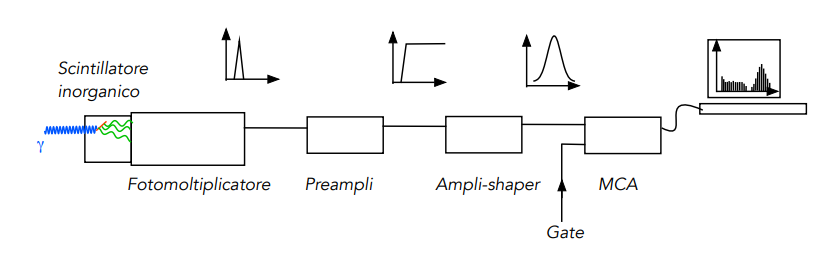
\includegraphics[scale=0.7]{Strumenti/electronic_chain.png} 
  \caption{In questa immagine è possibile visualizzare in maniera schematica la catena elettronica che caratterizza l'esperimento seguendo il segnale dal rivelatore alla sua digitalizzazione.}
  \label{fig:elettronica}
\end{figure}
\section{Apparato Sperimentale}
L'apparato sperimentale, visibile schematicamente nella fig. \ref{fig:apparato_sperimentale} è quindi costituito da:
\begin{itemize}
    \item Uno scintillatore inorganico cilindrico ai cristalli di $\ch{NaI} (\ch{Tl})$ accoppiato ad un fotomoltiplicatore;
    \item uno scintillatore inorganico cilindrico ai cristalli di $\ch{BeCr_3}$ accoppiato ad un fotomoltiplicatore,
    \item alimentatore ad alta tensione BERTAN Associates Model 313A che alimenta il fotomoltiplicatore accoppiato al rivelatore A,
    \item alimentatore ad alta tensione ORTEC 556 che alimenta il fotomoltiplicatore accoppiato al rivelatore B;
    \item due preamplitifacori SILENA che preamplificano il segnale uscente dai fotomoltiplicatori;
    \item amplificatore ORTEC AMP\&SCA 490A utilizzato per selezionare la finestra sul picco fotoelettrico per il gate;
    \item amplificatore ORTEC RESEARCH AMPLIFIER 450 utilizzato per formare il segnale da digitalizzare;
    \item un Multi-channel-Analyzer (MCA) inserito come scheda di espansione del PC utilizzato per acquisire lo spettro tramite il software MAESTRO;
    \item oscilloscopio Tektronix TDS 1002;
    \item modulo OPEN\_NIM che permette di effettuare i conteggi. 
\end{itemize}
 %IMMAGINE apparato_sperimentale
\begin{figure}[htp!]
  \centering
  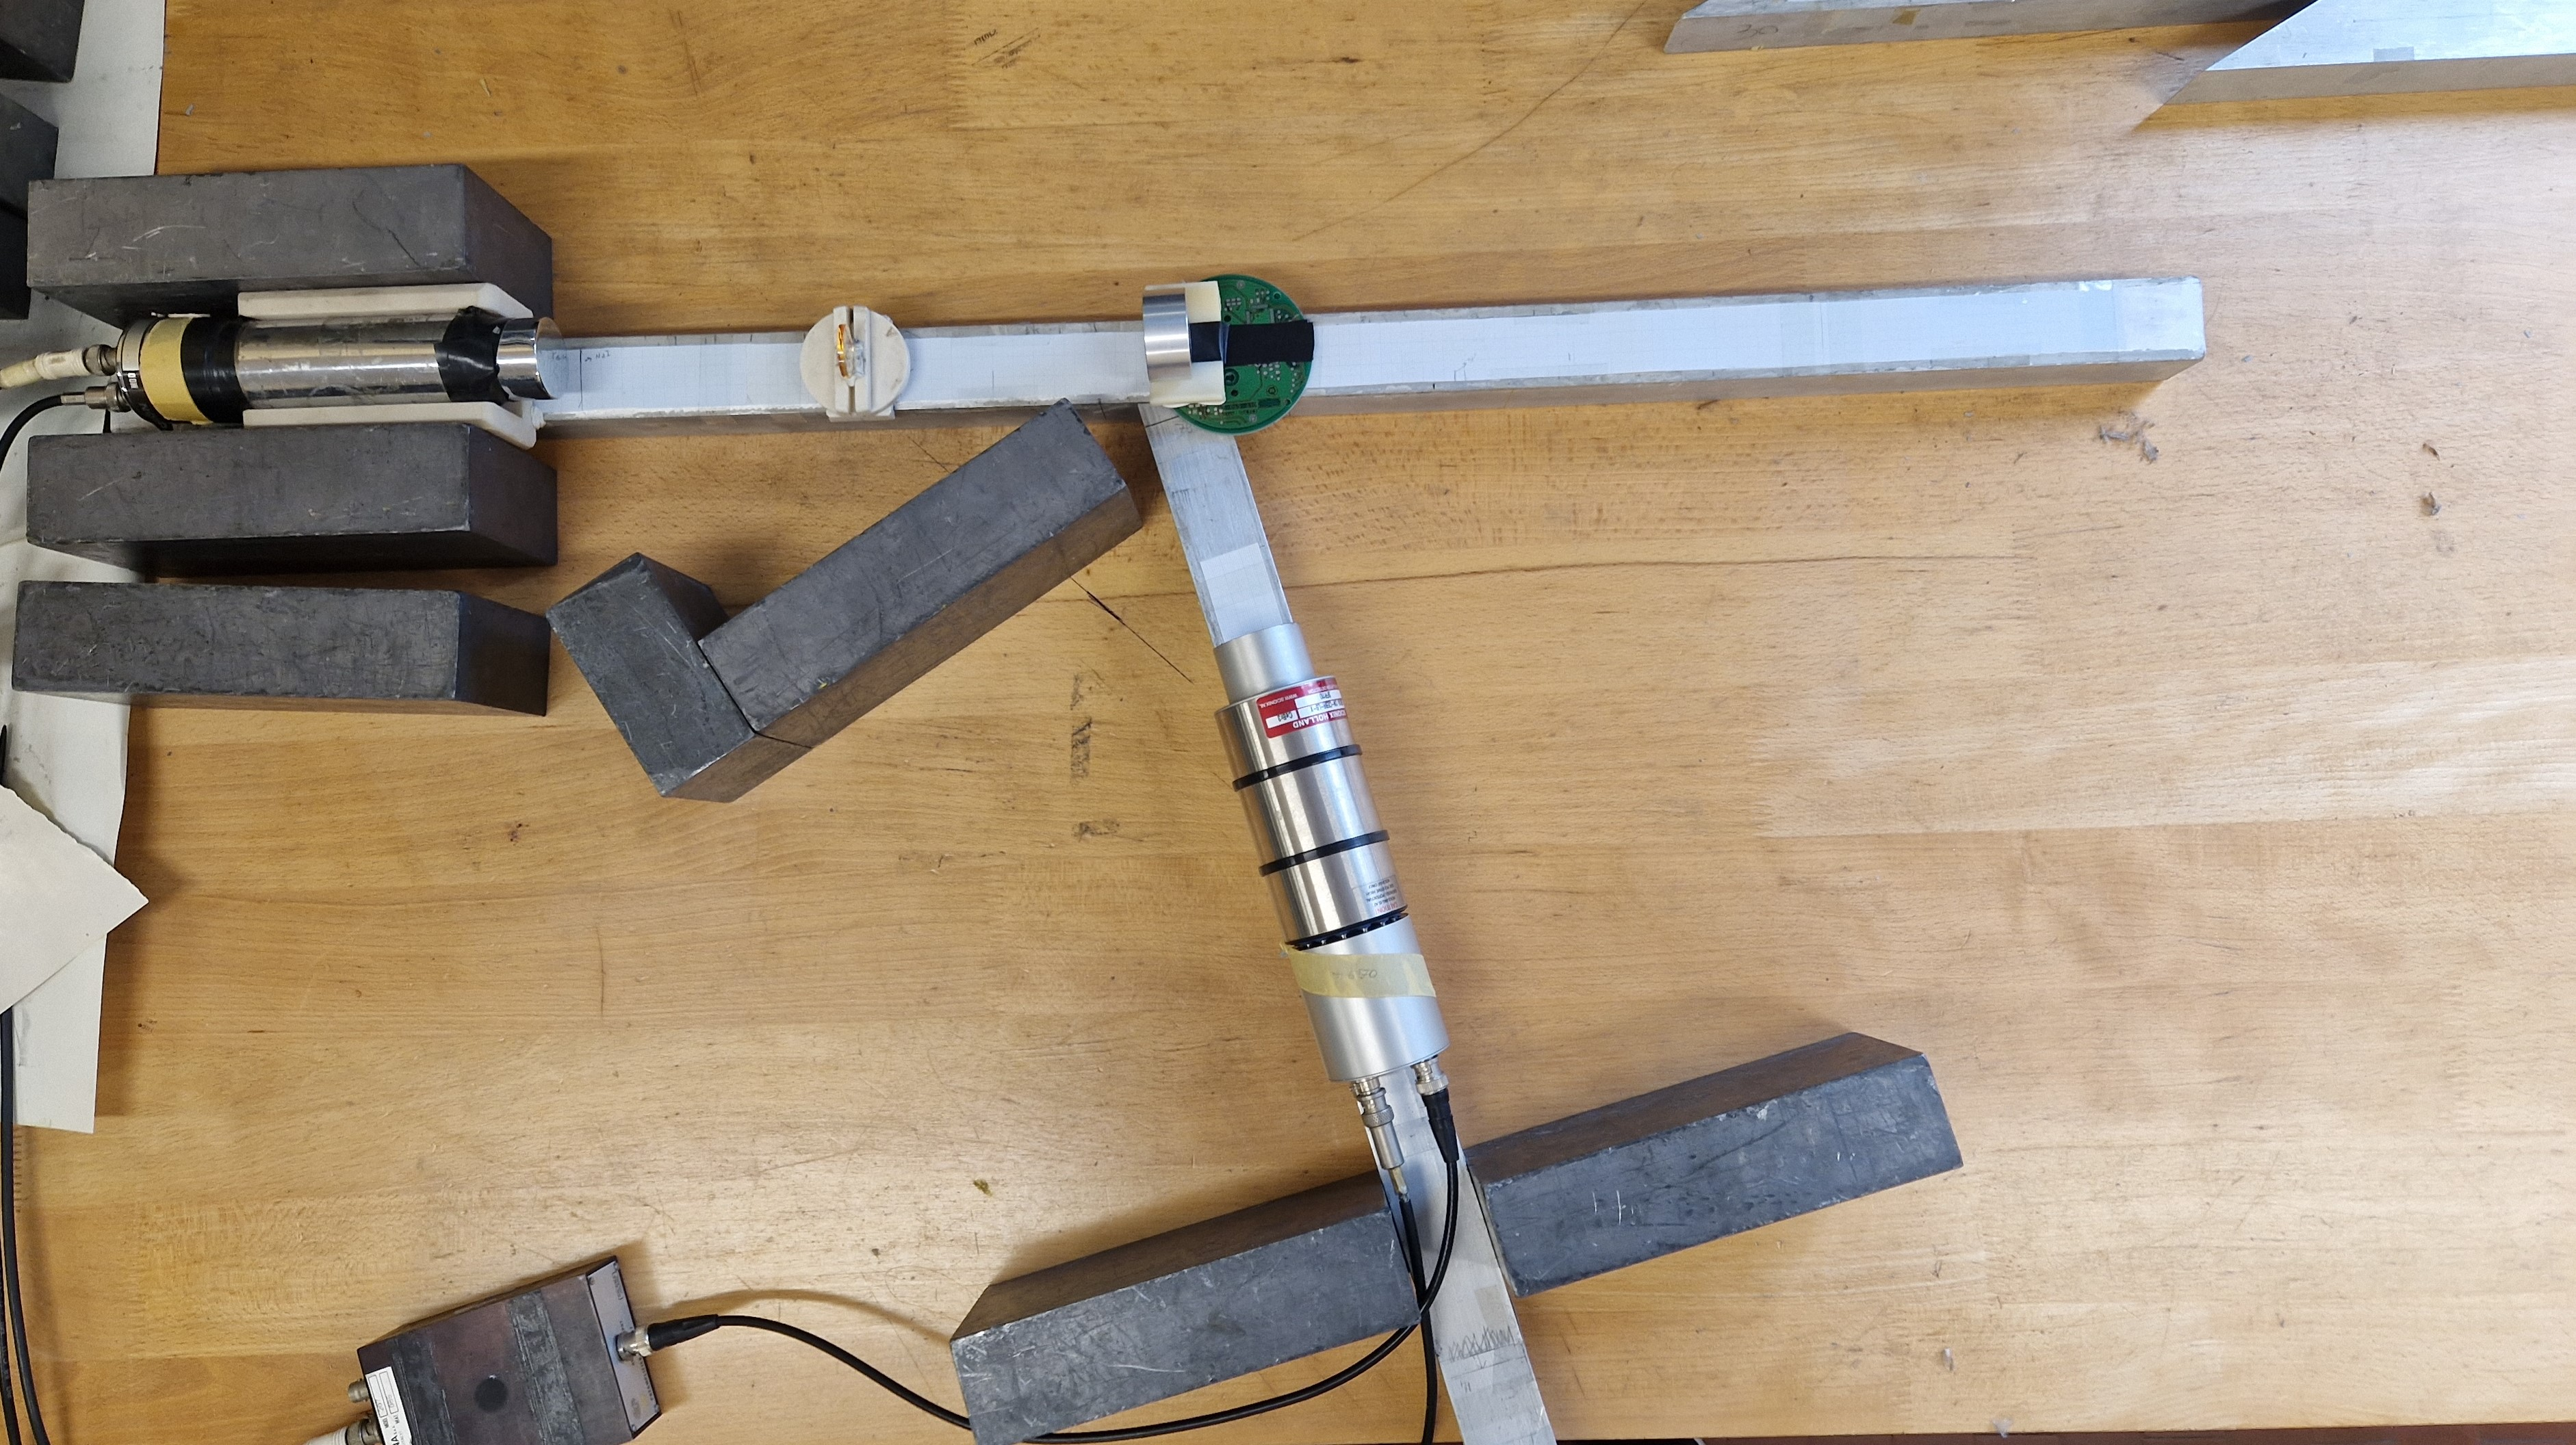
\includegraphics[scale=0.09]{Strumenti/apparato_sperimentale.jpg} 
  \caption{In questa immagine è possibile visualizzzare lo schema e la disposizione dell'apparato sperimentale durante una presa dati. Un'importante attenzione nei blocchi di $\ch{Pb}$ utilizzati sia per fissare i supporti ma anche per schermare i fotoni provenienti direttamente dalla sorgente.}
  \label{fig:apparato_sperimentale}
  %magari aggiungere delle didascalie all'interno dell'immagine o sostituire la foto con un disegno schematico
\end{figure}
Per assicurare un posizionamento stabile e preciso dei rivelatori, sono stati utilizzati dei supporti in metallo intagliati. Questi supporti hanno anche lo scopo di variare l'angolo di misura. Per quanto riguarda la sorgente e lo scatteratore, sono stati impiegati ulteriori supporti che hanno permesso un allineamento quantitativo di tutto il setup sperimentale. Tale allineamento è cruciale per minimizzare gli errori sistematici e ottenere dati affidabili. Le distanze sono scelte in modo che l'angolo solido sotteso allo scintillatore sia uguale rispetto all'angolo solido opposto che si forma con lo scatteratore. Oltre a questo è stata scelta una distanza molto maggiore rispetto ai raggi dei rivelatori in modo tale da porre l'apparato in buona geometria in modo da rendere trascurabile la frazione di radiazione secondaria che lo possa raggiungere. Ulteriori riflessioni sullo schema geometrico sono state affrontate in sezione \ref{sez_err_angolo_solido}
\subsection{Scelta del bersaglio}
Durante la fase preliminare dell'esperienza ci è stata data completa libertà sulla scelta del bersaglio. La selezione del materiale del bersaglio è stata effettuata considerando l'equazione che descrive il numero di fotoni scatterati:
\begin{equation}
     N_s = N_i \rho \frac{N_A}{M} Z dx \sigma(E)
     \label{eq:N_s}
\end{equation}
dove $\sigma$ è la sezione d'urto valutata per fotoni a $511\,\unit{keV}$, $N_s$ è il numero di fotoni scatterati, $N_i$ è il numero di fotoni incidenti, $\rho$ è la densità, $N_A$ la costante di Avogadro, $M$ è la massa molare del materiale, $Z$ è il numero atomico e $dx$ è lo spessore del bersaglio. I tre materiali presi in considerazione sono: alluminio, carbonio e rame.

A partire dai dati ottenuti attraverso il sito NIST XCOM\footnote{National Istitute of Standards and Technology: \url{https://physics.nist.gov/PhysRefData/Xcom/html/xcom1.html}} sono state fatte le seguenti considerazioni: per prima cosa, il rame è stato escluso poiché il contributo dell'effetto fotoelettrico è di un ordine di grandezza superiore rispetto a quello dell'alluminio e del carbonio, come è possibile visualizzare della tabella \ref{tab:bersagli}. Questo comporta che una significativa parte dei fotoni incidenti verrebbe assorbita piuttosto che scatterata, riducendo l'efficacia del bersaglio per lo scopo dell'esperimento.

\begin{table}[H]
    \centering
    \begin{tabular}{|c c c c|}
    \hline
    Elemento & $\sigma_{C}$ [\unit{\cm^{2}}] & $\sigma_{PH}$ [\unit{\cm^2}] & $\frac{\sigma_{C}}{\sigma_{TOT}}$ \\ [0.5ex] 
 \hline\hline
 Al & \num{2.860e-25} & \num{4.37e-28} & 99.19\% \\ 
 \hline
 C & \num{2.865e-25} & \num{2.15e-29} & 99.81\% \\ 
 \hline
 Cu & \num{2.848e-25} & \num{8.83e-27} & 94.67\% \\
 \hline 
    \end{tabular}
    \caption{Sezioni d'urto Compton (C) e Fotoelettrica (PH).}
    \label{tab:bersagli}
\end{table}
Successivamente è stato confrontato il carbonio e l'alluminio. Utilizzando l'equazione \ref{eq:N_s} è stato fatto un confronto tra il rapporto dei fotoni scatterati e incidenti con l'alluminio e il carbonio ottenendo i risultati visibili nella tebella (\ref{tab:considerazioni_finali}). Queste considerazioni ci hanno portato alla scelta finale dell'alluminio come bersaglio ottimale.
\begin{table}[H]
    \centering
    \begin{tabular}{|c c c c|}
    \hline
     Elemento & $\frac{N_s}{N_i}$ & $n_t dx \sigma$ & $\lambda_{COMP} [\unit{\cm}]$ \\ [0.5ex] 
 \hline\hline
 Al & 42.89\% & 0.4323 & 4.463 \\ 
 \hline
 C & 39.18\% & 0.392 & 5.117 \\ 
 \hline 
    \end{tabular}
    \caption{Confronto tra i fotoni scatterati utilizzando l'alluminio e il carbonio a parità di spessore ed energia dei fotoni.}
    \label{tab:considerazioni_finali}
\end{table}
Per quanto riguarda le dimensioni del bersaglio si è deciso di adottare come scatteratore un cilindro di alluminio di spessore pari a $2\, \unit{cm}$, che è circa la metà del valore di libero cammino medio dell'effetto Compton. La scelta di questa dimensione è dettata da due considerazioni principali: 
\begin{itemize}
    \item Massimizzare il rapporto $\frac{N_s}{N_i}$: un bersaglio con uno spessore sufficiente per ottenere un buon numero di fotoni scatterati, mantenendo un alto rapporto tra fotoni scatterati e incidenti.
    \item Assicurare un bersaglio sottile: mantenere $n_t \sigma dz << 1$ per evitare interazioni multiple e ridurre gli effetti di assorbimento all'interno del materiale. Un bersaglio sottile minimizza le probabilità di interazioni multiple dei fotoni con gli elettroni del bersaglio, garantendo che la maggior parte dei fotoni scatterati provengano da un singolo evento di scattering Compton.
\end{itemize}
Il bersaglio è stato intagliato da un cilindro di alluminio $6082$ utilizzando un tornio all'interno dell'officina nel dipartimento di fisca. L'alluminio serie $6000$ è anche conosciuto come anticorodal. 
\subsection{Geometria dell'apparato}
 Dal punto di vista sperimentale, le sezioni d'urto sono determinate per un angolo solido finito $\Delta \Omega$, che corrisponde all'angolo solido occupato dalla base del rivelatore cilindrico. L'angolo solido con cui un rivelatore di raggio $a$ "vede" una sorgente puntiforme posta a una distanza $d$ è dato da:
\begin{equation}
    \Omega=2\pi\left(1-\frac{d}{\sqrt{d^2+a^2}}\right)
\end{equation}
per $d>>a$ si approssima con:
\begin{equation}
    \Omega=\pi\frac{a^2}{d^2}
    \label{eq:angolo_solido}
\end{equation}
Le distanze tra i due rivelatori con la sorgente sono state quindi scelte in modo tale da eguagliare l'angolo solido sotteso. Questa configurazione assicura che ciascun rivelatore copra un volume angolare equivalente, migliorando la simmetria e la coerenza delle misure. Sono state fatte ulteriori considerazioni cercando di massimizzare l'efficienza di rivelazione studiata nella sezione dedicata \ref{eff}.
